%%%%%%%%%%%%%%%%%%%%%%%%%%%%%%%%%%%%%%%%%
% Beamer Presentation
% LaTeX Template
% Version 1.0 (10/11/12)
%
% This template has been downloaded from:
% http://www.LaTeXTemplates.com
%
% License:
% CC BY-NC-SA 3.0 (http://creativecommons.org/licenses/by-nc-sa/3.0/)
%
%%%%%%%%%%%%%%%%%%%%%%%%%%%%%%%%%%%%%%%%%

%----------------------------------------------------------------------------------------
%	PACKAGES AND THEMES
%----------------------------------------------------------------------------------------

\documentclass[9pt]{beamer}
\usepackage{CJK}
\usepackage{ctex}
\usepackage{graphicx}
\usepackage{subfigure}
\usepackage{longtable}
\usepackage{rotating}
\usepackage{multirow}
\usepackage{algorithm}
\usepackage{algorithmic}
\usepackage{mathtools}
\usepackage{animate}
%\usepackage{media9}
%% A LATEX package for embedding interactive Adobe Flash (SWF) and 3D files (Adobe U3D & PRC) as well as video and sound files or streams (FLV, MP4/H.246, MP3) into PDF documents with Adobe Reader-9/X
%compatibility.
\renewcommand{\algorithmicrequire}{\textbf{Input:}}   %Use Input in the format of Algorithm
\renewcommand{\algorithmicensure}{\textbf{Output:}}  %UseOutput in the format of Algorithm
\newcommand{\e}[1]{\ensuremath{\times 10^{#1}}}
%\mode<presentation>{\usetheme{Madrid}}

\mode<presentation> {

% The Beamer class comes with a number of default slide themes
% which change the colors and layouts of slides. Below this is a list
% of all the themes, uncomment each in turn to see what they look like.

%\usetheme{default}
%\usetheme{AnnArbor}
%\usetheme{Antibes}
%\usetheme{Bergen}
%\usetheme{Berkeley}
%\usetheme{Berlin}
%\usetheme{Boadilla}
%\usetheme{CambridgeUS}
%\usetheme{Copenhagen}
%\usetheme{Darmstadt}
%\usetheme{Dresden}
%\usetheme{Frankfurt}
%\usetheme{Goettingen}
%\usetheme{Hannover}
%\usetheme{Ilmenau}
%\usetheme{JuanLesPins}
%\usetheme{Luebeck}
\usetheme{Madrid}
%\usetheme{Malmoe}
%\usetheme{Marburg}
%\usetheme{Montpellier}
%\usetheme{PaloAlto}
%\usetheme{Pittsburgh}
%\usetheme{Rochester}
%\usetheme{Singapore}
%\usetheme{Szeged}
%\usetheme{Warsaw}

% As well as themes, the Beamer class has a number of color themes
% for any slide theme. Uncomment each of these in turn to see how it
% changes the colors of your current slide theme.

%\usecolortheme{albatross}
\usecolortheme{beaver}
%\usecolortheme{beetle}
%\usecolortheme{crane}
%\usecolortheme{dolphin}
%\usecolortheme{dove}
%\usecolortheme{fly}
%\usecolortheme{lily}
%\usecolortheme{orchid}
%\usecolortheme{rose}
%\usecolortheme{seagull}
%\usecolortheme{seahorse}
%\usecolortheme{whale}
%\usecolortheme{wolverine}

%\setbeamertemplate{footline} % To remove the footer line in all slides uncomment this line
%\setbeamertemplate{footline}[page number] % To replace the footer line in all slides with a simple slide count uncomment this line

%\setbeamertemplate{navigation symbols}{} % To remove the navigation symbols from the bottom of all slides uncomment this line
}

\usepackage{graphicx} % Allows including images
\usepackage{booktabs} % Allows the use of \toprule, \midrule and \bottomrule in tables
\begin{document}
\begin{CJK*}{GBK}{kai}
%----------------------------------------------------------------------------------------
%	TITLE PAGE
%----------------------------------------------------------------------------------------

\title[Machine Learning]{The Perceptron} % The short title appears at the bottom of every slide, the full title is only on the title page

\author{Kun He (����)} % Your name
%\logo{%
%   
\includegraphics[scale=.2]{logo.pdf}\hspace*{4.75cm}~%
%   
\includegraphics[scale=.2]{logo.jpg}\hspace*{0.75cm}%
%   }
%\pgfdeclareimage[width=1cm]{hust}{logo.pdf}
%\logo{\pgfuseimage{hust}{\vspace{-10pt}}}
\titlegraphic{
\includegraphics[width=1.3cm]{logo.pdf}}
\institute[JHL, HUST] % Your institution as it will appear on the bottom of every slide, may be shorthand to save space
{
	Data Mining and Machine Learning Lab\\
	(John Hopcroft Lab)\\
	Huazhong University of Science \& Technology \\ % Your institution for the title page
	\medskip
	\textit{brooklet60@hust.edu.cn} % Your email address
}

\date{2022��05��} % Date, can be changed to a custom date
%====================================================
\frame{\titlepage}

\frame{\frametitle{Table of Contents}\tableofcontents}

\AtBeginSection[]
{
\begin{frame}{Table of Contents}
\tableofcontents[currentsection]
\end{frame}
}

%------------------------------------------------
%------------------------------------------------
\section{Concept}
%------------------------------------------------
\subsection{Assumptions}
\begin{frame}
\frametitle{Assumptions}
\begin{block}{Assumptions}%{Basic idea:}
	\begin{itemize}
	\item Binary classification (i.e. $y_i \in \{-1, +1\}$)
	\item Data is linearly separable
	\end{itemize}	
\end{block}
\begin{figure}[h]
	\centering
	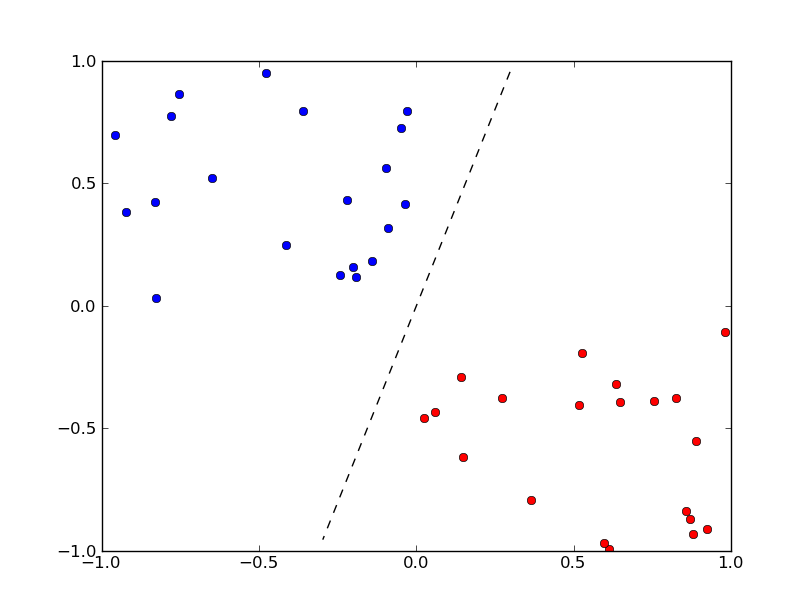
\includegraphics[scale=0.2]{Example.png}
\end{figure}
\end{frame}

\begin{frame}
	\frametitle{Assumptions}
	\begin{block}{Basic idea:}
	\begin{itemize}
	\item 
	In machine learning, the perceptron is an algorithm for supervised learning of binary classifiers.	
	\item 
	A binary classifier is a function which can decide whether or not an input, represented by a vector of numbers, belongs to some specific class.
	\item 
	It is a type of linear classifier, i.e. a classification algorithm that makes its 
		predictions based on a linear predictor function combining a set of weights with the feature vector.
	\end{itemize}	
	\end{block}
\centering
$\mathcal{H} = \{h(x) = \mathbf{w}^\top \mathbf{x} + b = 0 \}$
	
	\begin{figure}[h]
		\centering
		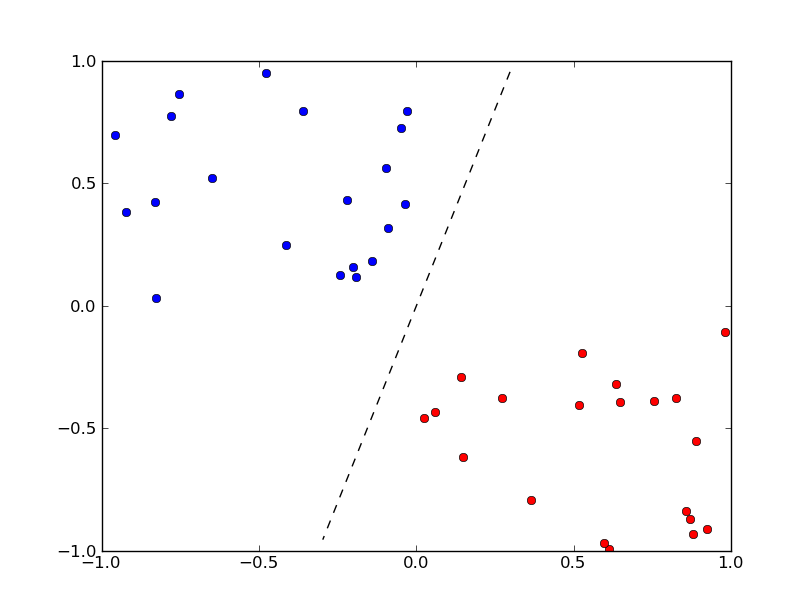
\includegraphics[scale=0.1]{Example.png}
	\end{figure}
\end{frame}
%------------------------------------------------
%------------------------------------------------
\section{Classifier}
%------------------------------------------------
\subsection{Parameter Selection}
\begin{frame}
\frametitle{Parameter Selection}
\centering
$h(x_i) = \textrm{sign}(\mathbf{w}^\top \mathbf{x}_i + b)$
 
\begin{figure}[h]
	\centering
	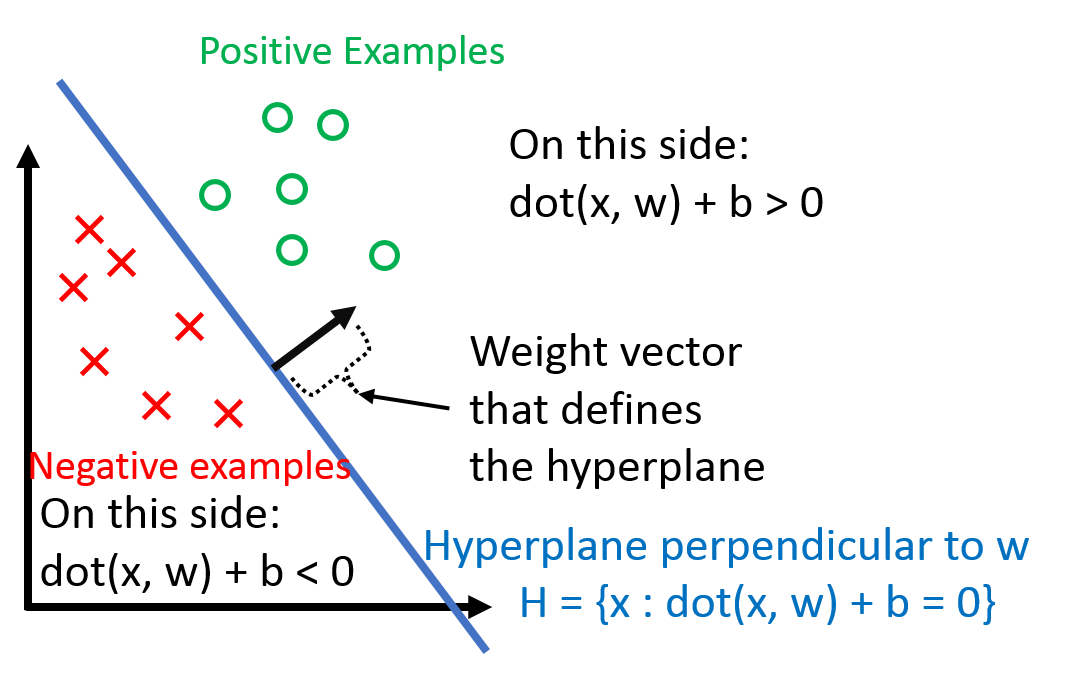
\includegraphics[scale=0.25]{perceptron_img1.png}
\end{figure}

\end{frame}
%------------------------------------------------
\begin{frame}
\frametitle{Parameter Selection}
$b$ is the bias term (without the bias term, the hyperplane that $\mathbf{w}$ defines would always have to go through the origin). Dealing with $b$ can be a pain, so we 'absorb' it into the feature vector $\mathbf{w}$ by adding one additional constant dimension. Under this convention,\\
\begin{center}
	$\mathbf{x}_i \hspace{0.1in} \text{becomes} \hspace{0.1in} \begin{bmatrix} \mathbf{x}_i \\ 1  \end{bmatrix} $\\
	\quad \\
	$\mathbf{w} \hspace{0.1in} \text{becomes} \hspace{0.1in} \begin{bmatrix} \mathbf{w} \\ b  \end{bmatrix} $\\
\end{center}
We can verify that\\
%\begin{center}
$\begin{bmatrix} \mathbf{x}_i \\ 1  \end{bmatrix}^\top \begin{bmatrix} \mathbf{w} \\ b  \end{bmatrix} = \mathbf{w}^\top \mathbf{x}_i + b $
%\end{center}
\\
Hence, \\
$\mathcal{H} = \{h(x) = \mathbf{w}^\top \mathbf{x} = 0 \}$
\end{frame}
%------------------------------------------------
\subsection{Hyperplane}
\begin{frame}
\frametitle{Hyperplane}
Then, we can simplify the above formulation of $h(\mathbf{x}_i)$ to
\begin{center}
	$h(\mathbf{x}_i) = \textrm{sign}(\mathbf{w}^\top \mathbf{x})$
\end{center}

\begin{figure}[h]
	\centering
	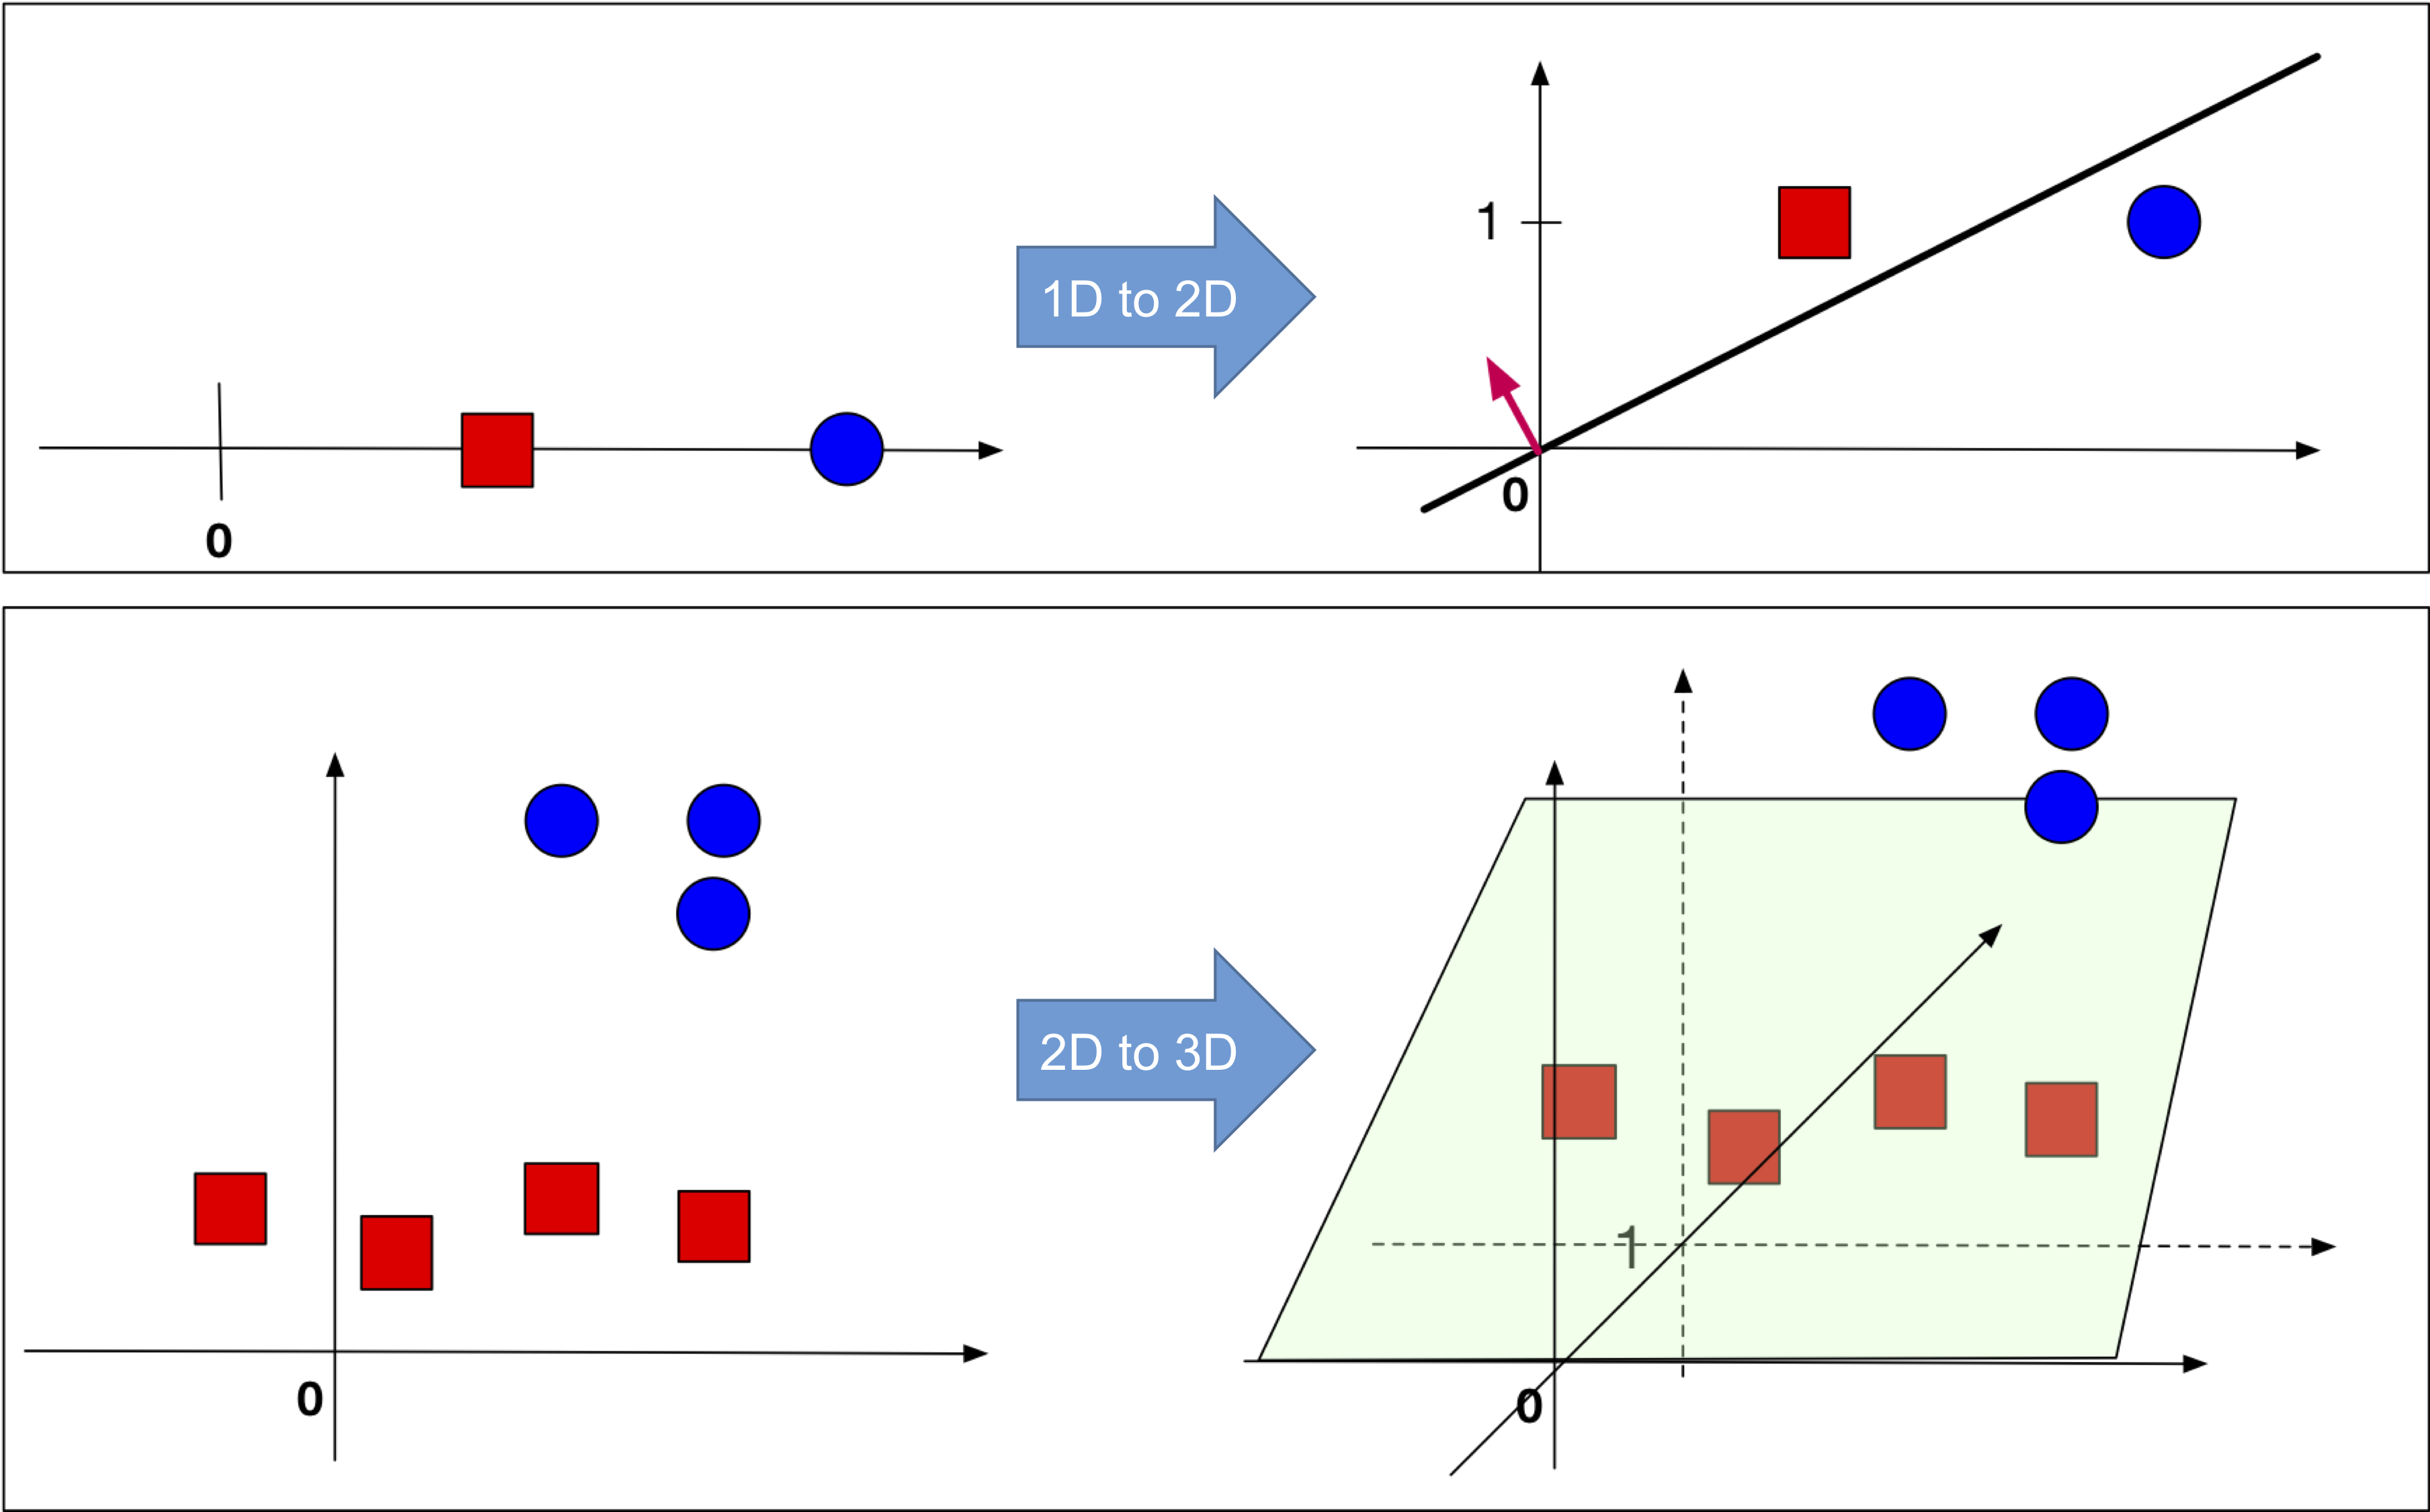
\includegraphics[scale=0.1]{PconstantDim}
\end{figure}
(Left:) The original data is 1-dimensional (top row) or 2-dimensional (bottom row). There is no hyper-plane that passes through the origin and separates the red and blue points. \\
(Right:) After a constant dimension was added to all data points, such a hyperplane exists.

\end{frame}
%------------------------------------------------
\begin{frame}
\frametitle{Hyperplane}
\begin{block}{Observation}
	Note that
	\begin{center}
		$y_i(\mathbf{w}^\top \mathbf{x}_i) > 0 \Longleftrightarrow \mathbf{x}_i \hspace{0.1in} \text{is classified correctly}$
	\end{center}
	where 'classified correctly' means that $x_i$ is on the correct side of the hyperplane defined by $\mathbf{w}$. Also, note that the left side depends on $y_i \in \{-1, +1\}$(it wouldn't work if, for example $y_i \in \{0, +1\}$).
\end{block}
\end{frame}
%%------------------------------------------------


%%------------------------------------------------
\section{Perceptron Algorithm}
%------------------------------------------------
\subsection{Algorithm}
\begin{frame}
\frametitle{Algorithm}
Now that we know what the $\mathbf{w}$ is supposed to do (defining a hyperplane that separates the data), let's look at how we can get such $\mathbf{w}$. 
\begin{figure}
	\centering
	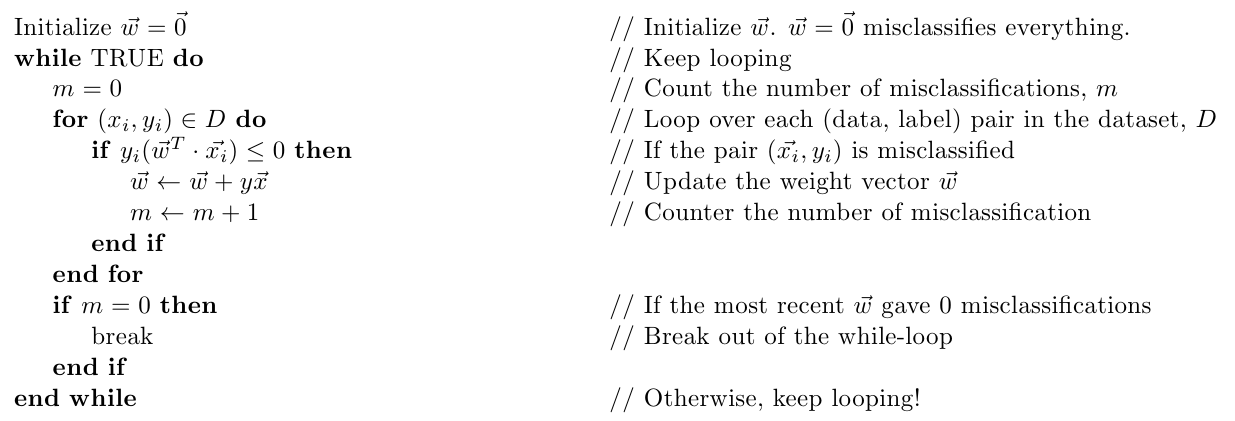
\includegraphics[scale=0.27]{perceptron_algo}
\end{figure}
\end{frame}
%------------------------------------------------
\subsection{Geometric Intuition}
\begin{frame}
\frametitle{Geometric Intuition}
\begin{figure}
	\centering
	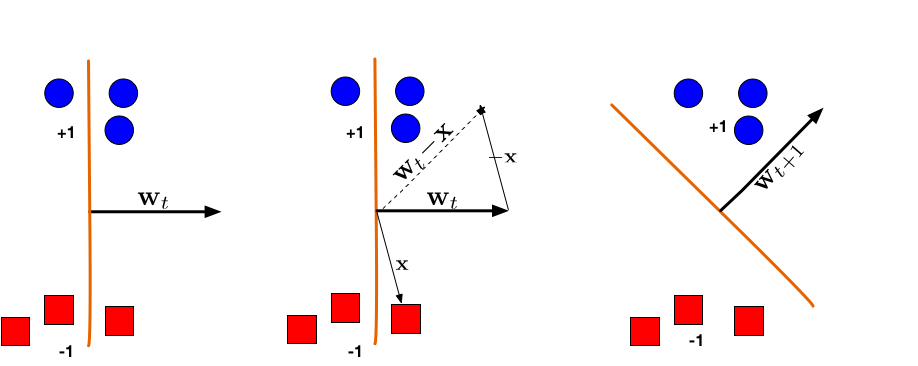
\includegraphics[scale=0.3]{PerceptronUpdate.png}
\end{figure}
Illustration of a Perceptron update.(Left:) The hyperplane defined by $\mathbf{w}_t$ misclassifies one red (-1) and one blue (+1) point. (Middle:) The red point $\mathbf{x}$ is chosen and used for an update. Because its label is -1 we need to $\mathbf{subtract~~x}$ from $\mathbf{w}_t$. (Right:) The udpated hyperplane $\mathbf{w}_{t+1}=\mathbf{w}_t-\mathbf{x}$ separates the two classes and the Perceptron algorithm has converged.
\end{frame}
%------------------------------------------------
\begin{frame}
\frametitle{Geometric Intuition}
\begin{block}{Quiz}
	Assume a data set consists only of a single data point $\{(\mathbf{x},+1)\}$. How often can a Perceptron misclassify this point $\mathbf{x}$ repeatedly? \\
	What if the initial weight vector $\mathbf{w}$ was initialized randomly and not as the all-zero vector?
\end{block}
\end{frame}

%------------------------------------------------
\section{Perceptron Convergence}
%------------------------------------------------
\subsection{Perceptron Convergence}
\begin{frame}
\frametitle{Perceptron Convergence}

The Perceptron was arguably the first algorithm with a strong formal guarantee. If a data set is linearly separable, the Perceptron will find a separating hyperplane in a finite number of updates. (If the data is not linearly separable, it will loop forever.)\\
\quad \\
The argument goes as follows: Suppose $\exists \mathbf{w}^*$ such that $y_i(\mathbf{x}^\top \mathbf{w}^*  ) > 0 $ $\forall (\mathbf{x}_i, y_i) \in D $ \\
\quad \\
Now, suppose that we rescale each data point and the $\mathbf{w}^*$ such that
\begin{center}
	$||\mathbf{w}^*|| = 1 \hspace{0.3in} \text{and} \hspace{0.3in} ||\mathbf{x}_i|| \le 1 \hspace{0.1in} \forall \mathbf{x}_i \in D $
\end{center}
\end{frame}
%------------------------------------------------
\begin{frame}
\frametitle{Perceptron Convergence}
Let us define the \underline{Margin $\gamma$ of the hyperplane} $\mathbf{w}^*$ as $\gamma = \min_{(\mathbf{x}_i, y_i) \in D}|\mathbf{x}_i^\top \mathbf{w}^*   |$.
\begin{figure}[h]
	\centering
	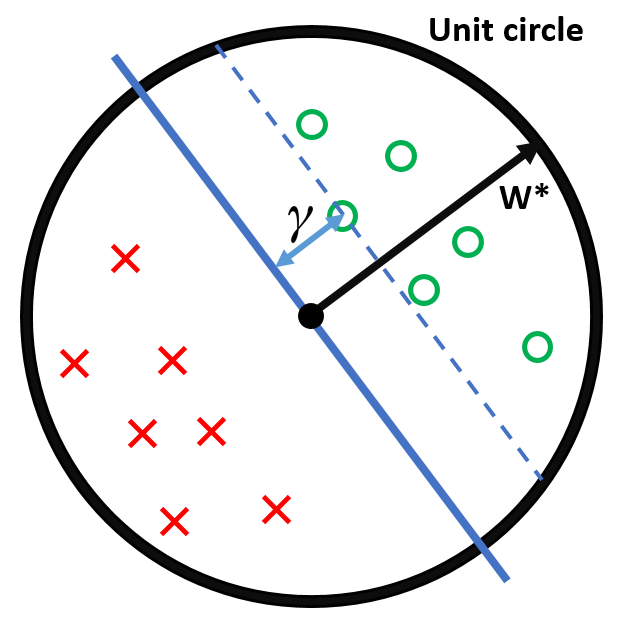
\includegraphics[scale=0.2]{perceptron_img3}
\end{figure}
To summarize our setup:\\
\begin{itemize}
	\item All inputs $\mathbf{x}_i$ live within the unit sphere
	\item There exists a separating hyperplane defined by $\mathbf{w}^*$, with $\|\mathbf{w}\|^*=1$ (i.e. $\mathbf{w}^*$ lies exactly on the unit sphere).
	\item $\gamma$ is the distance from this hyperplane (blue) to the closest data point.
\end{itemize}
\end{frame}
%------------------------------------------------
\subsection{Theorem and Proof}
\begin{frame}
\frametitle{Theorem and Proof}
\textbf{Theorem: }If all of the above holds, then the perceptron algorithm makes at most $1 / \gamma^2$ mistakes. \\
\quad \\
\textbf{Proof: }
Keeping what we defined above, consider the effect of an update ($\mathbf{w}$ becomes $\mathbf{w}+y\mathbf{x}$) on the two terms $\mathbf{w}^\top \mathbf{w}^*$ and $\mathbf{w}^\top \mathbf{w}$. We will use two facts:\\
\begin{itemize}
	\item $y( \mathbf{x}^\top  \mathbf{w})\leq 0$: This holds because $\mathbf{x}$ is misclassified by $\mathbf{w}$ - otherwise we wouldn't make the update.
	\item $y( \mathbf{x}^\top  \mathbf{w}^*)>0$: This holds because $\mathbf{w}^*$ is a separating hyper-plane and classifies all points correctly.
\end{itemize}
\end{frame}
%------------------------------------------------
\begin{frame}
\frametitle{Theorem and Proof}
1.Consider the effect of an update on $\mathbf{w}^\top \mathbf{w}^*$: 
\begin{center}
	$(\mathbf{w} + y\mathbf{x})^\top \mathbf{w}^* = \mathbf{w}^\top \mathbf{w}^* + y(\mathbf{x}^\top  \mathbf{w}^*) \ge \mathbf{w}^\top \mathbf{w}^* + \gamma$
\end{center}
The inequality follows from the fact that, for $\mathbf{w}^*$, the distance from the hyperplane defined by $\mathbf{w}^*$ to $\mathbf{x}$ must be at least $\gamma$ (i.e. $y (\mathbf{x}^\top  \mathbf{w}^*)=|\mathbf{x}^\top \mathbf{w}^*|\geq \gamma$). 
\quad \\
\underline{This means that for each update}, $\mathbf{w}^\top \mathbf{w}^*$ \underline{grows by \textbf{at least }$\gamma$.}
\quad \\
\quad \\
2.Consider the effect of an update on $\mathbf{w}^\top \mathbf{w}$:
\begin{center}
	$(\mathbf{w} + y\mathbf{x})^\top   (\mathbf{w} + y\mathbf{x}) = \mathbf{w}^\top \mathbf{w} + \underbrace{2y(\mathbf{w}^\top\mathbf{x})}_{<0} + \underbrace{y^2(\mathbf{x}^\top  \mathbf{x})}_{0\leq \ \ \leq 1} \le \mathbf{w}^\top \mathbf{w} + 1$
\end{center}
The inequality follows from the fact that
\begin{itemize}
	\item $2y(\mathbf{w}^\top  \mathbf{x}) < 0$ as we had to make an update, meaning $\mathbf{x}$ was misclassified
	\item $0\leq y^2(\mathbf{x}^\top  \mathbf{x}) \le 1$as $y^2 = 1$ and all $\mathbf{x}^\top  \mathbf{x}\leq 1$ (because $\|\mathbf x\|\leq 1$).
\end{itemize}
\underline{This means that for each update}, $\mathbf{w}^\top \mathbf{w}$ \underline{grows by \textbf{at most 1}.}
\end{frame}
%------------------------------------------------
\begin{frame}
\frametitle{Theorem and Proof}
3.Now we can put together the above findings. Suppose we had $M$ updates.
\begin{align}
	M\gamma &\le \mathbf{w}^\top \mathbf{w}^* &&\text{By first point} \\
	&= |\mathbf{w}^\top \mathbf{w}^*| &&\text{Simply because $M\gamma \geq 0$} \\
	&\le ||\mathbf{w}||\  ||\mathbf{w}^*|| &&\text{By Cauchy-Schwartz inequality$^*$} \\
	&= ||\mathbf{w}|| &&\text{As $||\mathbf{w}^*|| = 1$} \\
	&= \sqrt{\mathbf{w}^\top \mathbf{w}} && \text{by definition of $\|\mathbf{w}\|$} \\
	&\le \sqrt{M} &&\text{By second point} \\ 
	& \textrm{ }\\
	&\Rightarrow M\gamma \le \sqrt{M} \\
	&\Rightarrow M^2\gamma^2 \le M \\
	&\Rightarrow M \le \frac{1}{\gamma^2}
\end{align}
And hence, the number of updates $M$ is bounded from above by a constant.\\
\quad\\
$^*$Alternative explanation:$|\mathbf{w}^\top\mathbf{w}^*|=\|\mathbf{w}\|\|\mathbf{w}^*\||\cos(\alpha)|$, but $|\cos(\alpha)|\leq 1$
\end{frame}
%------------------------------------------------
\begin{frame}
\frametitle{Theorem and Proof}
\begin{block}{Quiz}
	Given the theorem above, what can you say about the margin of a classifier (what is more desirable, a large margin or a small margin?) Can you characterize data sets for which the perceptron algorithm will converge quickly? Draw an example.
\end{block}
\end{frame}

%------------------------------------------------
\section{Perceptron in the History}
%------------------------------------------------
\subsection{Perceptron History}
\begin{frame}
	\frametitle{Perceptron in the History}
	\begin{itemize}
	\item The perceptron algorithm was invented in 1957 at the Cornell Aeronautical Laboratory by \textbf{Frank Rosenblatt}.
	\item Mark I Perceptron machine, the first implementation of the perceptron algorithm. It was connected to a camera with $20 \times 20$ cadmium sulfide photocells(��ϸ������) to make a 400-pixel image. The main visible feature is a patch panel that set different combinations of input features. To the right, arrays of potentiometers(ǿ��������) that implemented the adaptive weights.
	\end{itemize}

	\begin{figure}[h]
	\centering		
	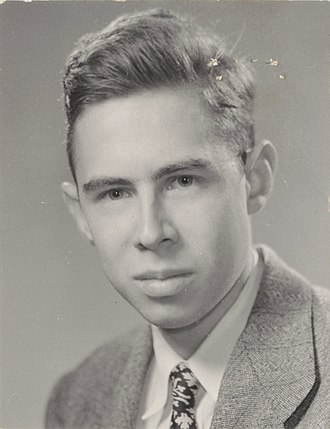
\includegraphics[scale=0.32]{FrankRosenblatt.png}~~~~~~~~~~	
	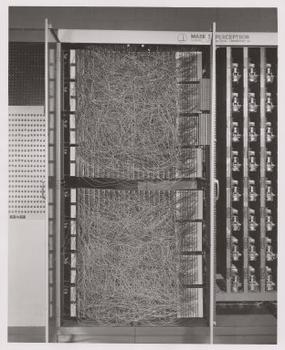
\includegraphics[scale=0.4]{MarkIPerceptronmachine.png}			
   \end{figure}
	%Do
\end{frame}


%------------------------------------------------
\begin{frame}
	\frametitle{Perceptron in the History}
	\begin{itemize}
		\item Initially, huge wave of excitement ("Digital brains") (See The New Yorker December 1958)
		\item Then, contributed to the A.I. Winter. Famous example of a simple non-linearly separable data set, the XOR problem (Minsky 1969):
	\end{itemize}		
	%\begin{block}{Examples of Feature Vectors}
	\begin{figure}[h]
		\centering	
		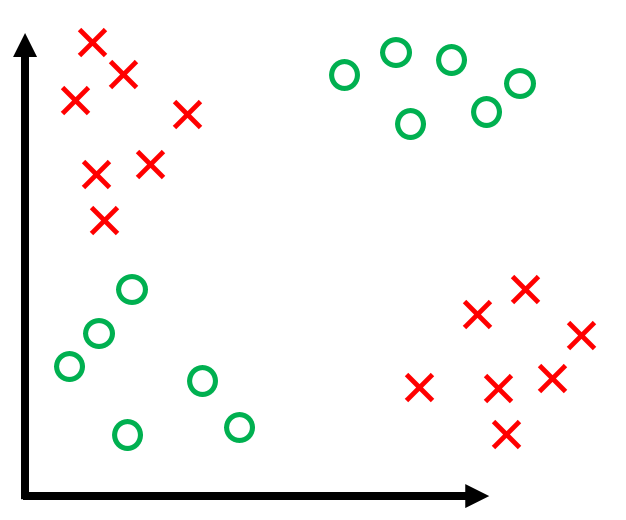
\includegraphics[scale=0.3]{XOR.png}			
	\end{figure}
	%\end{block}
	%Do
\end{frame}

%------------------------------------------------
\begin{frame}
	\frametitle{AND, OR, NOT, XOR}	
	%\begin{block}{Examples of Feature Vectors}
	\begin{figure}[h]
		\centering	
		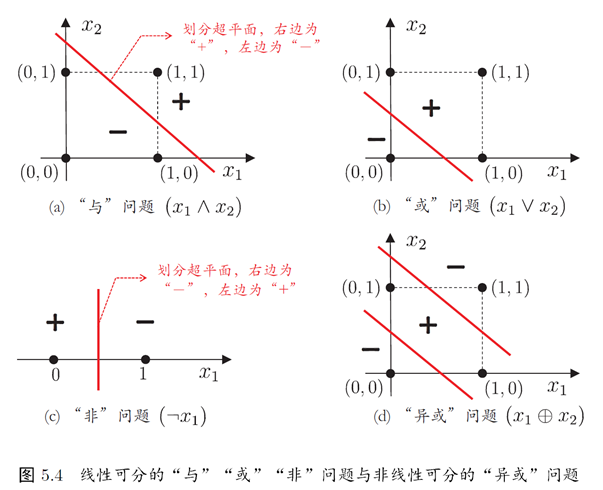
\includegraphics[scale=0.5]{AND-XOR.png}			
	\end{figure}
	%\end{block}
	%Do
\end{frame}

%------------------------------------------------
\subsection{From Perceptron to Artificial Neurons}
\begin{frame}
	\frametitle{Understanding the Perceptron as Neuron}
	\begin{itemize}
		\item The ��Mark 1 perceptron�� is machine was designed for image recognition: it had an array of 400 photocells(��ϸ������), randomly connected to the ``neurons".
		\item  Weights were encoded in potentiometers, and weight updates during learning were performed by electric motors.
	\end{itemize}
	
	\begin{figure}[h]
		\centering		
		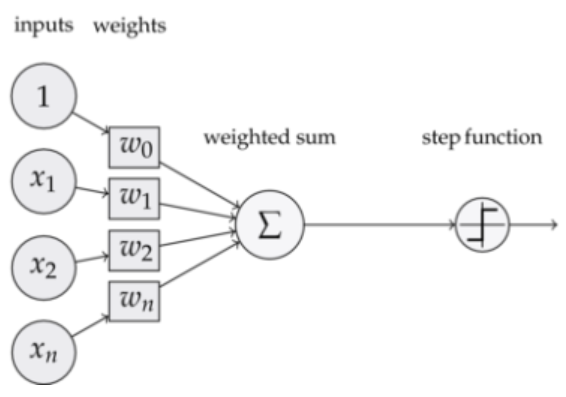
\includegraphics[scale=0.32]{Perception2Neuron.png}			
	\end{figure}
	%Do
\end{frame}

%------------------------------------------------
%\subsection{From Perceptron to Artificial Neurons}
\begin{frame}
	\frametitle{From Perceptron to Neurual Network}
	\begin{itemize}
		\item  \textbf{Input}: All the feature becomes the input for a perceptron, $x = [x_1, x_2, ...,x_n] $.  
		\item \textbf{Weights}: Weights are the values that are computed over the time of training the model. Initial we start the value of weights with some initial value and these values get updated for each training error. $w =[w_1,w_2,... w_n]$.
		\item \textbf{BIAS}: A bias neuron allows a classifier to shift the decision boundary left or right. In an algebraic term, the bias neuron allows a classifier to translate its decision boundary. BIAS helps to training the model faster and with better quality.
		\item \textbf{Weighted Summation}: Weighted Summation is the sum of value that we get after the multiplication of each weight associated the each feature value. 
		\item \textbf{Step/Activation Function}: the role of activation functions is make neural networks non-linear. %For linerarly classification of example, it becomes necessary to make the perceptron as linear as possible.
		\item \textbf{Output}: The weighted Summation is passed to the step/activation function and whatever value we get after computation is our predicted output.  
	\end{itemize}
	
	\begin{figure}[h]
		\centering		
		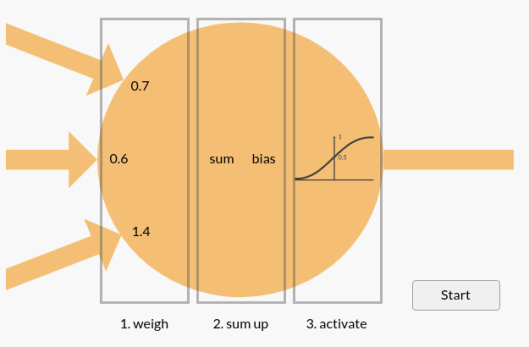
\includegraphics[scale=0.3]{InsidePerceptron.png}			
	\end{figure}
	%Do
\end{frame}

%------------------------------------------------
\iffalse
\section{Perceptron Example Code}
\begin{frame}
	\frametitle{Perceptron Example Code}
	\centering
	\href{https://github.com/IEC-lab/MachineLearning2019/blob/master/Perceptron/perceptron.py}{Click here: Perceptron example python code}
\end{frame}
\fi 
%%------------------------------------------------
\section{Reference}
%------------------------------------------------
\begin{frame}
\frametitle{Reference}
\begin{thebibliography}{4}
\bibitem{CS4780} https://www.cs.cornell.edu/courses/cs4780/2018fa/page18/
\end{thebibliography}
\end{frame}
%%------------------------------------------------
%\section{Reference}
%------------------------------------------------
%\begin{frame}
%\frametitle{Reference}
%\begin{thebibliography}{4}
%\bibitem{LS-SPH} F. Zou, C. Liu, H. Ling, H. Feng, L. Yan, and D. Li, "Least square regularized spectral hashing for similarity search," Signal Processing, vol. 93, pp. 2265-2273, 2013. (SCI,EI)
%\bibitem{KMFH} F. Zou, Y. Chen, J. Song, K. Zhou, Y. Yang, and N. Sebe, "Compact image fingerprint via multiple kernel hashing," IEEE Transactions on Multimedia, vol. 17, pp. 1006-1018, 2015. (SCI,EI)
%\bibitem{KNPH} C. Liu, H. Ling, F. Zou, L. Yan, Y. Wang, H. Feng, et al., "Kernelized neighborhood preserving hashing for social-network-oriented digital fingerprints," IEEE Transactions on Information Forensics and Security, vol. 9, pp. 2232-2247, 2014. (SCI,EI)
%\bibitem{DTSH} Liu, Yu; Song, Jingkuan; Zhou, Ke; Yan, Lingyu; Liu, Li; Zou, Fuhao; Shao, Ling, "Deep Self-taught Hashing for Image Retrieval," IEEE Transactions on Cybernetics, May 3, 2018. (SCI,EI)
%\bibitem{DeepFace} Fuhao Zou, Fan Yang, Wei Chen,Kai Lia, Jingkuan Song, Jingcai Chen, Hefei Ling, "Fast Large Scale Deep Face Search," Pattern Recognition Letters, Januray 3, 2019. (SCI,EI)
%\end{thebibliography}
%\end{frame}
%------------------------------------------------
\begin{frame}
\Huge{\centerline{The End}}
\end{frame}
\end{CJK*}
\end{document}
%\end{document}
